\documentclass[13pt]{article}
\usepackage[utf8]{inputenc}
\usepackage{polski}
\usepackage{amsmath}%matma
\usepackage{graphicx}%zdjecia
\usepackage{siunitx}
\usepackage{a4wide}
\graphicspath{{./figures/}}
\usepackage[framemethod=TikZ]{mdframed}
\usepackage{array,tabularx}
\usepackage{pythontex}

\renewcommand*\descriptionlabel[1]{\hspace\leftmargin$#1$}
\newcommand{\definebox}[2]{%
  \newcounter{#1}
  \newenvironment{#1}[1][]{%
    \stepcounter{#1}%
    \mdfsetup{%
        frametitle={%
            \tikz[baseline=(current bounding box.east),outer sep=0pt]
            \node[anchor=east,rectangle,fill=white]
            {\strut \MakeUppercase#1~\csname the#1\endcsname\ifstrempty{##1}{}{:~##1}};}}%
    \mdfsetup{innertopmargin=1pt,linecolor=#2,%
        linewidth=2pt,topline=true,
        frametitleaboveskip=\dimexpr-\ht\strutbox\relax,}%
    \begin{mdframed}[]\relax%
    }{\end{mdframed}}%
}

\definebox{definicja}{black!60}

\title{Analiza i synteza przebiegów odkształconych - szeregi Fouriera}
\author{Mikołaj Małecki 237339 K00-15c}
\begin{document}
	\maketitle
\section{Wprowadzenie}
Szereg Fouriera jest to ciąg (dla danej chwili t) wyrażony wzorem:
\begin{definicja}[Szereg Fouriera]
$$x(t) = a_0 + \sum_{k=1}^{\infty}(a_k \cos(k \omega_0 t) + b_k \sin(k \omega_0 t))$$
gdzie:
\begin{description}
\item[a_0] - wartość średnia - jego zmiana powoduje offset sugnału estymowaneg
\item[a_k , b_k] - współczynniki trygonometryczne - ich odpowiednie dobranie pozwala z pewną dokładnością estymować sygnały
\end{description}
\end{definicja}
Dla czasu niedyskretnego operacja wyliczenia wartości z powyższej definicji oznacza nałożenie na siebie kolejnych skłądowych harmonicznych estymowanego sygnału. Dla nieskończonego ciągu sumy waryżeń szeregu - wynik jest równy estymowanemu sygnałowi. Jednakże z uwagi na niemożliwość przeprowadzenia takiej operacji numerycznie dobiera się wartość liczby wyrazów sumy optymalnie pod względem kryterium potrzebnej dokłądności do uciążliwości wykonywanych obliczeń.

\begin{figure}[!h]
	\centering
	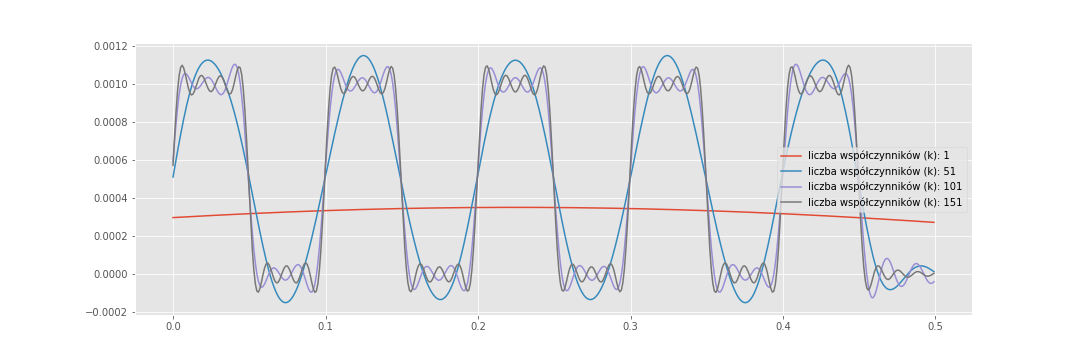
\includegraphics[width=\textwidth]{example.png}
	\caption{Sygnał binarny unipolarny estymowany szeregami fouriera z różną liczbą współczynników}
\end{figure}

\newpage

Można zauważyć że kolejne wykresy przedstawiające bardziej dokładne estymacje coraz bardziej ukazują przebieg binarny. Co się stanie kiedy zwiększymy zmienną k ?

\begin{figure}[!h]
	\centering
	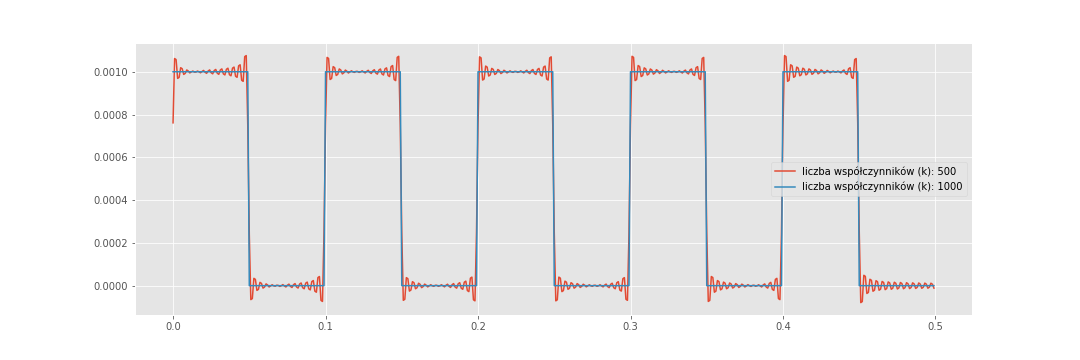
\includegraphics[width=\textwidth]{example2.png}
	\caption{Sygnał binarny unipolarny estymowany szeregami fouriera z różną liczbą współczynników}
\end{figure}

Można zauważyć że przebiegi dla odpowiednio większy wartości k w widocznym przybliżeniu nie odbiegają od oryginalnego. 
\\Jak natomiast wygląda sytuacja czasu obliczeń? Dla poniższych przebiegów:
\begin{figure}[!h]
	\centering
	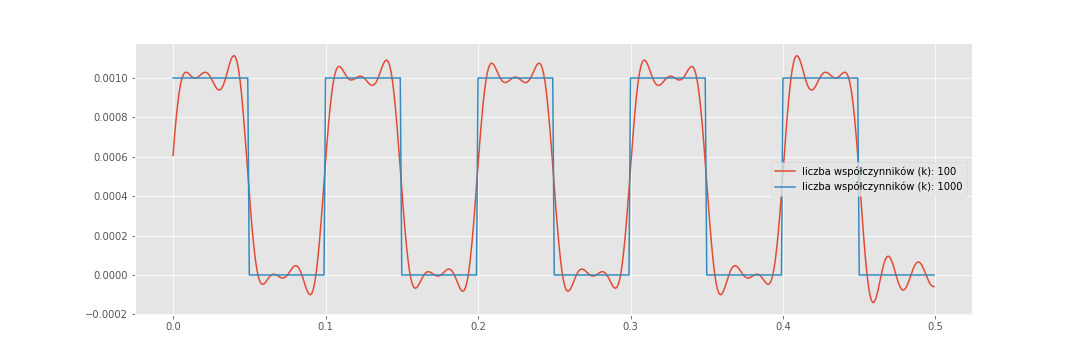
\includegraphics[width=\textwidth]{example3.png}
	\caption{Sygnał binarny unipolarny estymowany szeregami fouriera z różną liczbą współczynników}
\end{figure}

\begin{itemize}
\item Dla k = 10 $\rightarrow$ \texttt{100 loops, best of 3: 5.54 ms per loop}
\item Dla k = 1000 $\rightarrow$ \texttt{10 loops, best of 3: 55.9 ms per loop}
\end{itemize}

\newpage

\section{Przebiegi czasowe i ich estymacje}
\subsection{Kod}
\begin{itemize}
\item Dla wygenerowania żądanych przebiegów stworzony został generator sygnałów:
\begin{pyverbatim}
def make_func(func_L, func_R, amp, f):
    dx = 1
    time = np.arange(0, num_periods * f, dx)
    h_T = int(np.floor(len(time)/(num_periods*2)))
    func = np.zeros_like(time)

    for i in range(num_periods):
        func[i*2 * h_T : (i*2+1) * h_T] = func_L(h_T) * amp
        func[(i*2+1) * h_T : (i*2+2) * h_T] = func_R(h_T) * amp
    return Signal(time/1000, time/1000, func/1000, dx/1000)
\end{pyverbatim}

\item Natomiast w celu obliczenia współczynników potrzebnych do otrzymowania estymowanego sygnału utworzona została metoda:
\begin{pyverbatim}
def m_approx(signal, n_harmonics):
    A0 = np.sum(signal.y * np.ones_like(signal.x)) * signal.dx
    fFS = A0/2

    A = np.zeros(n_harmonics)
    B = np.zeros(n_harmonics)
    for k in range(n_harmonics):
        A[k] = np.sum(signal.y * np.cos(np.pi*(k+1)*signal.time)) * signal.dx
        B[k] = np.sum(signal.y * np.sin(np.pi * (k+1)*signal.time)) * signal.dx
        fFS += A[k]*np.cos(np.pi*(k+1)*signal.time) + B[k]*np.sin(np.pi * (k+1)*signal.time)
    return Signal(signal.time, signal.x, fFS, signal.dx)
\end{pyverbatim}

\item Wreszcie zestawienie żądanych wykresów zostało wykonane za pomocą funkcji:
\begin{pyverbatim}
def make_plots(signal: Signal, name: str, coefs: int):
    fig, ax = plt.subplots(2,2)

    ax[0, 0].plot(signal.x, signal.y, label=f"{name} - original")
    ax[0, 0].legend(loc="upper right")

    sig = m_approx(signal, coefs)
    ax[0, 1].plot(sig.x, sig.y, label=f"{name} - estimated")
    ax[0, 1].legend(loc="upper right")
    ax[1, 0].plot(sig.x, sig.y)
    ax[1, 0].plot(signal.x, signal.y, label=f"{name} - both")
    ax[1, 0].legend(loc="upper right")

    ax[1, 1].plot(sig.x, sc.fft(sig.y), label=f"fft")
    ax[1, 1].legend(loc="upper right")

    plt.show(fig)
\end{pyverbatim}
\end{itemize}
\newpage

\subsection{Prostokąt}
\begin{pyverbatim}
L = lambda h_T: np.ones(h_T)
P = lambda h_T: np.zeros(h_T)
square = make_func(L,P,1,100)
make_plots(square, "square", 200)
\end{pyverbatim}
\begin{figure}[!h]
	\centering
	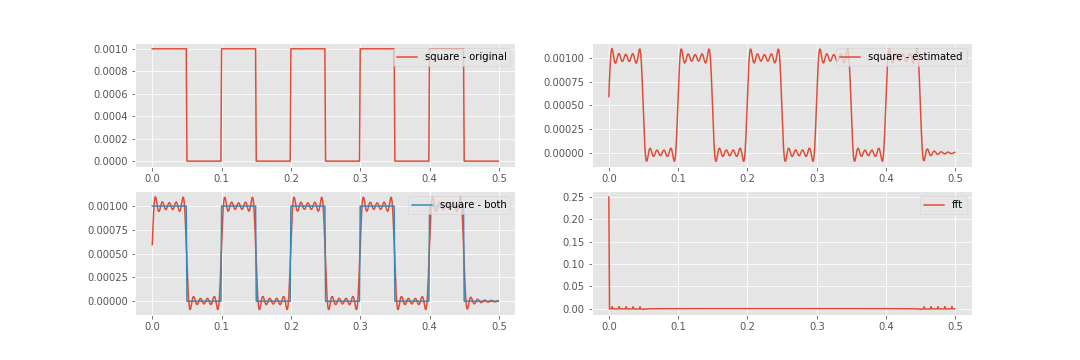
\includegraphics[width=\textwidth]{square.png}
	\caption{Zestaw przebiegów dla syngału prostokątnego}
\end{figure}

\subsection{Piła}
\begin{pyverbatim}
L = lambda h_T: np.arange(0, h_T)
P = lambda h_T: np.arange(0, h_T)
saw_tooth = make_func(L,P,1,100)
make_plots(saw_tooth, "saw_tooth", 200)
\end{pyverbatim}
\begin{figure}[!h]
	\centering
	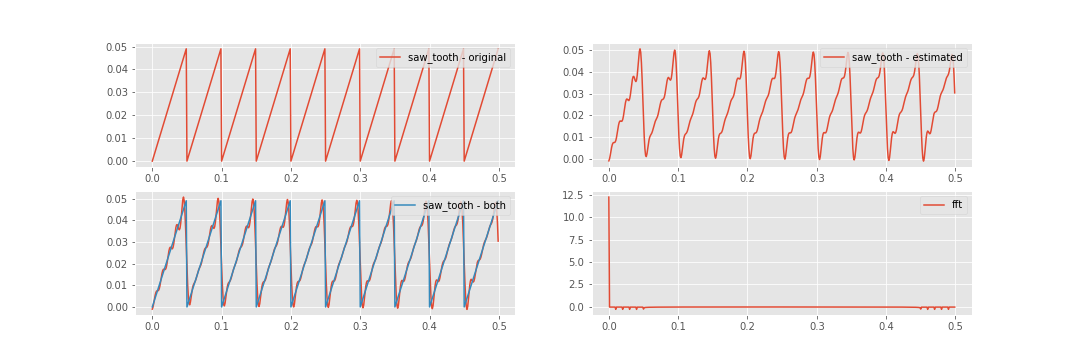
\includegraphics[width=\textwidth]{saw_tooth.png}
	\caption{Zestaw przebiegów dla syngału piły}
\end{figure}
\newpage


\subsection{Trapez}
\begin{pyverbatim}
L = lambda h_T: np.hstack([np.arange(0, h_T/2), np.ones(int(h_T/2))*int(h_T/2)])
P = lambda h_T: np.hstack([np.ones(int(h_T/2))*int(h_T/2), np.flipud(np.arange(0, h_T/2))])
trapeze = make_func(L,P,1,100)
make_plots(trapeze, "trapeze", 200)
\end{pyverbatim}
\begin{figure}[!h]
	\centering
	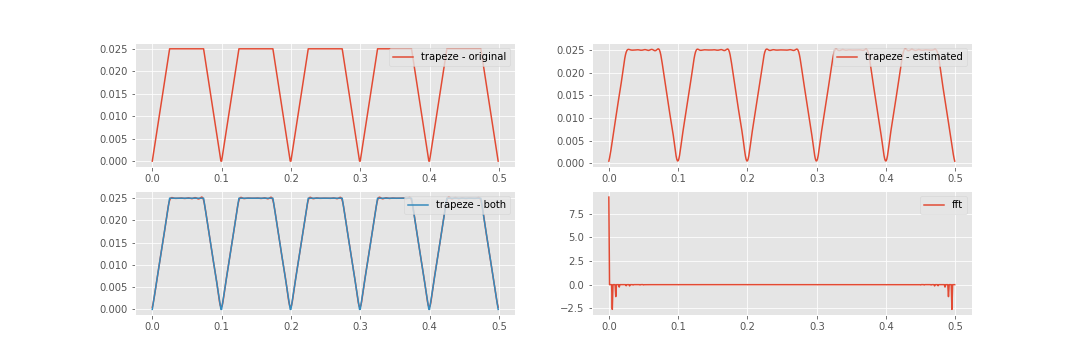
\includegraphics[width=\textwidth]{trapeze.png}
	\caption{Zestaw przebiegów dla syngału trapezoidalnego}
\end{figure}


\subsection{Trójkąt}
\begin{pyverbatim}
L = lambda h_T: np.arange(0, h_T)
P = lambda h_T: np.flipud(np.arange(0,h_T))
triangle = make_func(L,P,1,20)
make_plots(triangle, "triangle", 400)
\end{pyverbatim}
\begin{figure}[!h]
	\centering
	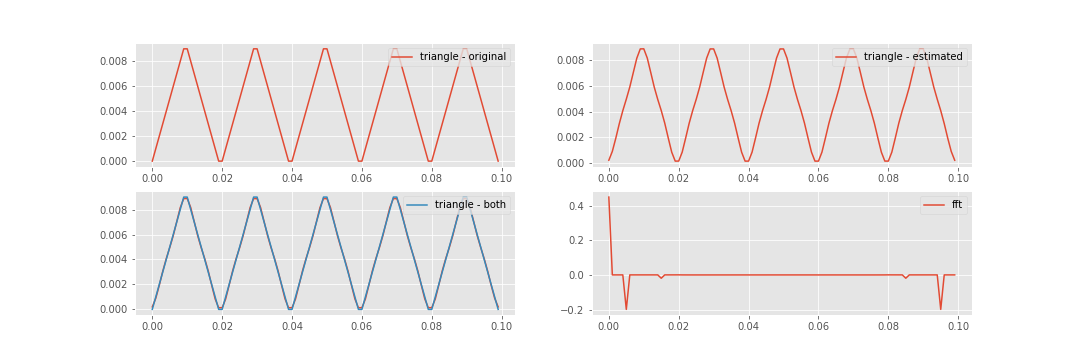
\includegraphics[width=\textwidth]{triangle.png}
	\caption{Zestaw przebiegów dla syngału trójkątnego}
\end{figure}

\newpage

\section{Obliczenia z wykorzystaniem zespolonego szeregu fouriera}
Bazując na wygodzie pracowania w dyskretnym środowisku programistycznym korzyść ze zmniejszenia liczby całkowań w tej metodzie nie jest adekwatna do złożoności zaprogramowania tej metody. Operacja całkowania dla dyskretnych skończonych danych jest poprostu operacją sumowania dlatego większość obliczeń została wykonana z podstawowej definicji.

Natomiast dla sygnału piłokształtnego, obliczenia z wykorzystaniem zespolonego szeregu fouriera przedstawiają się dla sygnału $\rightarrow$ \textbf{Rys.5} \textit{saw\_tooth - original} - sygnał piły w czasie.
$$A=0.05 \quad T=0.05s \quad f=20Hz \quad \omega_0=40 \pi \frac{rad}{s}$$
$$c_k = \int_{0}^{1} t \cdot e^{-jk \omega_0 t}dt = - \frac{e^{-2i \pi k}(-2i \pi k + e^{2i \pi k} - 1)}{4 \pi^2 k^2}$$
$$c_k = \frac{j}{2k \pi}$$
$$a_k = 2Re(c_k)=0 \quad b_k = -2Im(c_k) = \frac{-1}{k \pi} \quad a_0 = 0.05$$
Zatem sygnał można zapisać w postaci:
$$x_{ap}(t) = 0.05 + \sum_{k=1}^{k_0}(\frac{-1}{k \pi} \sin(40k \pi t))$$

\section{Wnioski}
\begin{itemize}
\item Wraz ze zwiększaniem liczby uwzględnianych harmonicznych dokładność estymacji rośnie
\item Wraz ze zwiększaniem liczby uwzględnianych harmonicznych efekt gibsa maleje (niestandardowo dla ostrych krawędzi sygnału bazowego)
\item Kolejne harmoniczne są widoczne jako skwantowane stałe wartości na widmie fazowym
\end{itemize}
\begin{thebibliography}{9}
\bibitem{lab} 
Instrukcja do laboratorium
\\\textit{Szeregi Fouriera}.

\bibitem{yt} 
3Blue1Brown
\\\textit{Ale czym jest szereg Fouriera? Od przepływu ciepła do szkiców okręgów}.
\\texttt{https://www.youtube.com/watch?v=r6sGWTCMz2k} 
\end{thebibliography}
\end{document}
